\section{Diagramme d'interaction : connexion}
\begin{figure}[H]
	\centering
	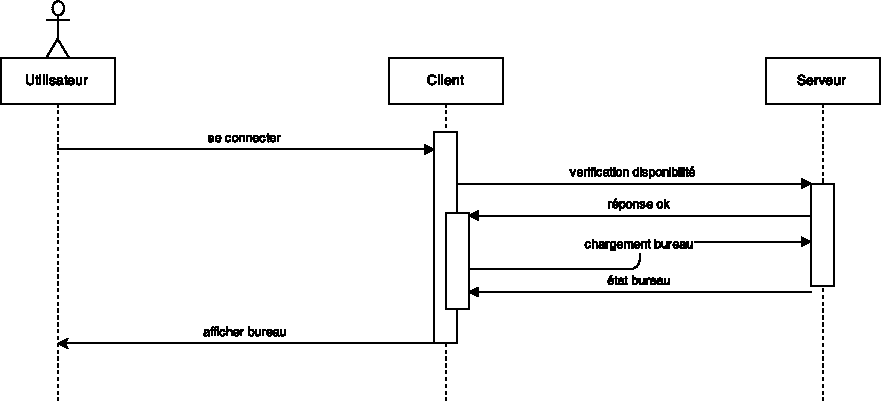
\includegraphics[angle=90]{diagrammes/DI1.pdf}
	\caption{\color{ForestGreen}Diagramme d'interaction : connexion (modifié)}
\end{figure}

\section{Diagramme d'interaction : déplacement de widget}
\begin{figure}[H]
	\centering
	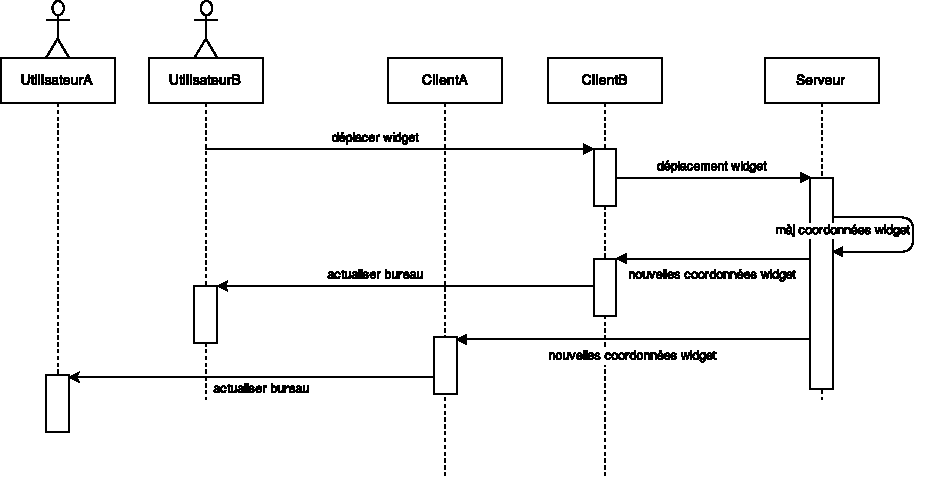
\includegraphics[angle=90]{diagrammes/DI2.pdf}
	\caption{\color{ForestGreen}Diagramme d'interaction : déplacement de widget (modifié)}
\end{figure}

\section{Diagramme d'interaction : déplacement de widget avec conflit}
\begin{figure}[H]
	\centering
	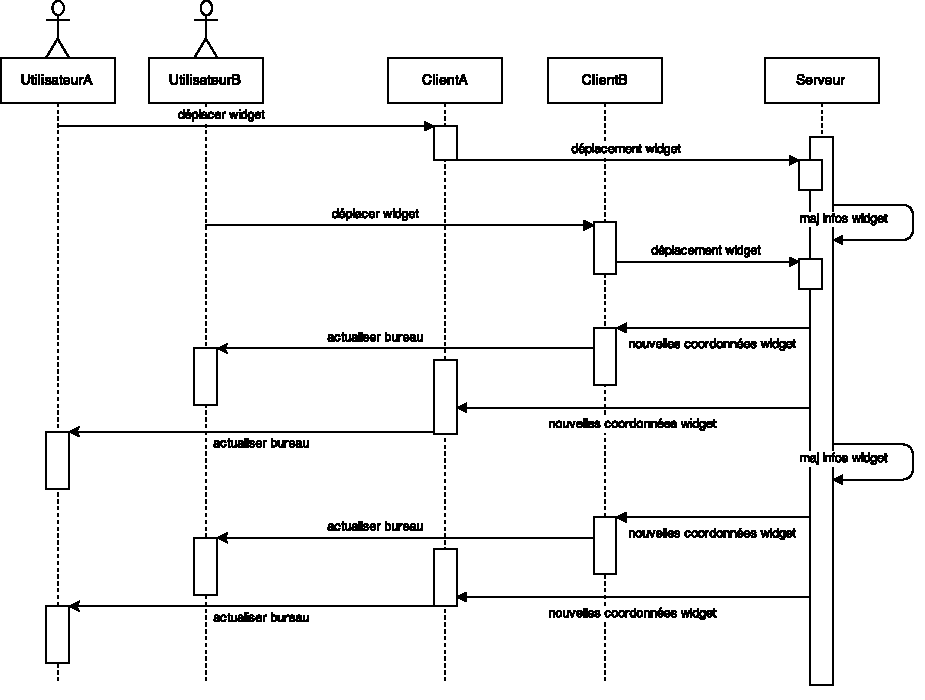
\includegraphics[angle=90]{diagrammes/DI3.pdf}
	\caption{\color{ForestGreen}Diagramme d'interaction : déplacement de widget avec conflit (modifié)\color{black}}
\end{figure}

\color{red}On voit ici que lorsqu'un utilisateur prend la main sur un widget, son état ne peut être modifié par un autre utilisateur.\color{black}

\color{ForestGreen}Les mises à jour par échange de l'état du bureau se faisant pratiquement en temps réel, la possibilité d'un conflit est réduite. Cependant, si un tel conflit prend place, nous avons décidé de ne pas gérer la priorité des utilisateurs sur les objets. Si un utilisateur saisit un objet et le déplace à lors qu'un autre utilisateur est en train de le déplacer, une première diffusion de l'état du bureau est faite (correspondant au premier utilisateur) puis une deuxième diffusion est faite (correspondant à l'état du bureau du second utilisateur ne prenant pas en compte la première diffusion). \color{black}